\def\figpath{tex/3_Kippschaltung/pictures}
\graphicspath{{tex/3_Kippschaltung/pictures/}}

\chapter{Kippschaltung}
Im 3. Kapitel werden astabile Kippschaltungen analysiert, welche, wie der Name schon sagt, keinen stabile Zustand besitzen und ohne äußere Erregung zwischen 2 Zuständen hin- und herschalten. 

\section{Astabile Kippstufe}
Zuerst wird ein Klassiker unter den elektronischen Schaltungen, und zwar der astabile Multivibrator, betrachtet. Analysiert wird die Schaltung lt. dem Schematic aus dem Praktikumsskript, Abb. \ref{fig_Kap3_01:Astab_Schem}. Diese Schaltung besteht aus zwei wechselseitig verbundenen elektronischen Schaltern, hier mithilfe von npn-Transistoren realisiert, und aus zwei RC-Gliedern, welche letztendlich die Schaltperiode bestimmen.

\begin{figure}[H]
    \centering
    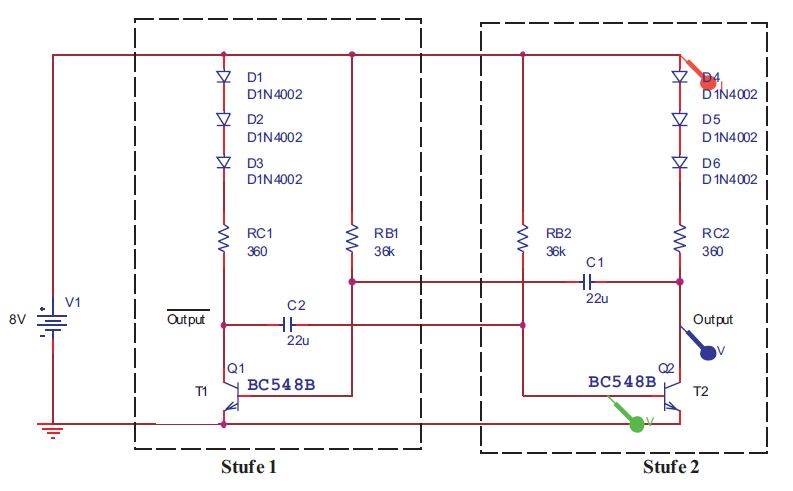
\includegraphics[width = 0.8\textwidth]{\figpath/Astabile_Kippschaltung_Schem.jpg}
    \caption{Astabile Kippschaltung}
    \label{fig_Kap3_01:Astab_Schem}
\end{figure}

\subsection{Analyse der Schaltung}
Die Kollektorwiderstände $R_{C1}$ und $R_{C2}$ begrenzen den Kollektorstrom des Transistors, die Basiswiderstände $R_{B1}$ und $R_{B2}$ müssen ein durchsteuern der Transistoren noch gewährleisten. Zunächst soll der Einschaltvorgang betrachtet werden. Die Schaltung wird vereinfacht (ohne Dioden) in Abb. \ref{fig_Kap3_02:Kipp_ESB} dargestellt. 

\begin{figure}[H]
	\centering
	\def\svgwidth{\textwidth}
	\input{\figpath/Kipp.pdf_tex}
	\caption{Reduziertes ESB der Kippschaltung} 
	\label{fig_Kap3_02:Kipp_ESB} 
\end{figure}


\subsubsection{Einschaltvorgang}
Ohne angelegter Versorgungsspannung sind die Kondensatoren $C_1$ und $C_2$ zunächst entladen, die Transistoren $T_1$ und $T_2$ sperren. Wird nun eine Betriebsspannung $U_B$ angelegt, fließt Strom einerseits über $R_{C1}$, $C_2$ und parallel durch $R_{B2}$ zur Basis von $T_2$, andererseits über $R_{C2}$, $C_1$ und parallel durch $R_{B1}$ zur Basis von $T_1$. Bauteiltoleranzen führen dazu, dass ein Transistor vor dem anderen durchschaltet. Zur einfacheren Erklärung wird nun die $T_1$ verbunden und sei zu diesem Zeitpunkt noch nicht geladen, wodurch das Potential der Basis von $T_2$ Richtung Masse gezogen wird und somit $T_2$ sperrt. Der Transistor $T_1$ bezieht seinen Basisstrom von $R_{B1}$ und $C_1$. Sollte sich $C_1$ bereits aufgeladen haben, liegt an seinen Klemmen ca. $U_B - U_{BE,1}$ an, da ja gilt: $I_{C2} = 0$. In der Zwischenzeit wird der Kondensator $C_2$ solange über den Widerstand $R_{B2}$ geladen, bis an der Basis von $T_2$ die Basis-Emitter-Durchlassspannung erreicht wird ($U_{BE,2} \approx 0,7$ V). Da die Kondensatoren zu diesem Zeitpunkt noch nicht vollständig geladen sind ist dieser Einschaltvorgang, wie sich auch in der Simulation zeigen wird, von kürzerer Dauer, als die Umschaltzeiten des eigentlichen periodischen Verhaltens.

\subsubsection{Periodisches Verhalten}
Zustand $T_1$ leitet: \\
Vor diesem Zustand war $T_1$ sperrend, womit $U_{CE,1}$ ungefähr $U_B$ betrug. Leitet nun $T_1$ sinkt die Kollektor-Emitterspannung auf $U_{CE,1,sat}$. Das Potential der kollektorseitigen Elektrode des Kondensators $C_2$ sinkt nun ebenso um $U_B - U_{CE,1,sat}$. Die Spannung an der gegenüberliegenden Elektrode von $C_2$, mit der Basis von $T_2$ verbunden, sinkt nun ebenso um denselben Betrag, da ja die Spannung am Kondensator bekanntlich nicht springen kann. Davor war $T_2$ leitend womit an dieser Elektrode die Durchlassspannung von ca. 0,7 V wirkte. Somit sinkt die Spannung an der Basis von $T_2$ um

\begin{equation}
U_{BE,2} \approx 0,7 - (U_B - U_{CE,1,sat}) = -U_B + U_{CE,1,sat} + 0,7 .
\end{equation}

Die Versorgungsspannung ist größer als die Sättigungs- und Durchlassspannungen am Transistor, womit die Basis-Emitterspannung negativ wird und $T_2$ sicher sperrt. Mit anderen Worten, die Polarität des Kondensators $C_2$ hat sich sprunghaft geändert. Das Potential an der kollektorseitigen Elektrode ist nun geringer als an der basisseitigen. Es startet ein Umladevorgang. $C_2$ lädt sich über $R_{B2}$ so lange auf, bis an der Basis von $T_2$ wieder jene Basis-Emitter-Durchlassspannung wirkt.

Zustand $T_2$ leitet: \\
Die Vorgänge finden umgekehrt zum vorhergehend erklärten Zustand statt. Die Kollektor-Emitterspannung von $T_2$ sinkt auf $U_{CE,2,sat}$, womit die Spannungen an den Klemmen von $C_1$ um $U_B - U_{CE,1,sat}$ sinken. 

\begin{equation}
U_{BE,1} \approx 0,7 - (U_B - U_{CE,2,sat}) = -U_B + U_{CE,2,sat} + 0,7 .
\end{equation}

Aufgrund der negativen Basis-Emitterspannung sperrt $T_1$ sicher. Nun wird $C_1$ über $R_{B1}$ geladen, bis $U_{BE,1} \approx 0,7$V gilt.

\subsubsection{Periodendauer}
Wann die Schaltungen die Zustände wechseln hängt somit von den Zeitkonstanten beider RC-Glieder ab.

\begin{equation}
    \tau_1 = R_{B1} \cdot C_1
\end{equation}

\begin{equation}
    \tau_2 = R_{B2} \cdot C_2
\end{equation}

Der Umladevorgang am Kondensator kann folgendermaßen beschrieben werden

\begin{equation}
    U_{C}(t) = U_{end} + (U_{start} - U_{end}) \cdot e^{-\frac{t}{\tau}}.
\end{equation}

Vernachlässigt man die Kollektor-Emitter-Sättigungsspannung gegenüber der Versorgungsspannung gilt

\begin{equation}
    U_{end} = U_B
\end{equation}

und 

\begin{equation}
    U_{start} = -U_B .
\end{equation}

Trifft man weiters die vereinfachende Annahme, dass der Transistor ab einer Basisspannung von 0V leitet, folgt

\begin{equation}
    U_{C}(T) = 0 = U_B - 2 U_B \cdot e^{-\frac{T}{\tau}}
\end{equation}

\begin{equation}
    \frac{1}{2} = e^{-\frac{T}{\tau}}
\end{equation}

\begin{equation}
    T = \text{ln}(2) \cdot \tau
\end{equation}

Die gesamte Periodendauer der betrachteten Kippschaltung bestimmt sich somit aus jener Zeitdauer, wo der Transistor $T_1$ leitet, 

\begin{equation}
    T_1 \approx \text{ln}(2) \cdot R_{B2}C_2 ,
\end{equation}

und jener wo Transistor $T_2$ leitet

\begin{equation}
    T_2 \approx \text{ln}(2) \cdot R_{B1}C_1 .
\end{equation}

Die betrachtete Schaltung ist symmetrisch, woraus sich eine Periodendauer von

\begin{equation}
    \label{glgn:period}
    T \approx 2 \cdot \text{ln}(2) \cdot R_{B1}C_1 = 2 \cdot \text{ln}(2) \cdot \SI{36}{\kilo\ohm} \cdot \SI{22}{\micro\farad} = \SI{1.098}{\second}
\end{equation}

ergibt.

Eine LED leuchtet für jene Dauer, in der ein bestimmter Transistor leitet, was bei der symmetrischen Schaltung die halbe Periode ist,

\begin{equation}
    T_{1,2} \approx \text{ln}(2) \cdot R_{B1}C_1 = 2 \cdot \text{ln}(2) \cdot \SI{36}{\kilo\ohm} \cdot \SI{22}{\micro\farad} = \SI{0.549}{\second}.
\end{equation}


\subsection{Simulation}
Die Schaltung wurde in LTSpice simuliert. Das zugehörige Schematic kann in Abb. \ref{fig_Kap3_03:LTSpice_Schem_1} betrachtet werden.

\begin{figure}[H]
    \centering
    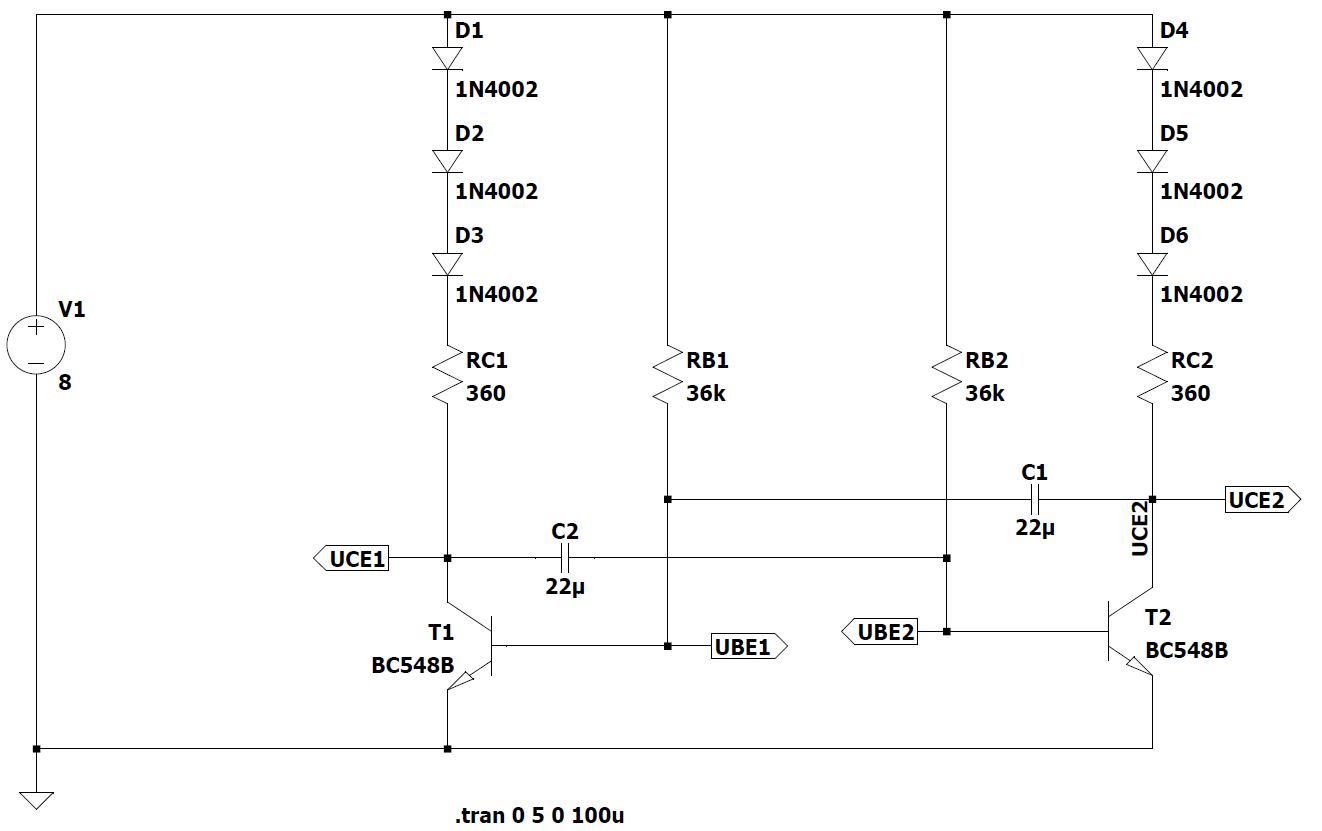
\includegraphics[width = 0.8\textwidth]{\figpath/Kipp_schem_1.jpg}
    \caption{Astabile Kippschaltung in LTSpice}
    \label{fig_Kap3_03:LTSpice_Schem_1}
\end{figure}

Es wurde eine 5 Sekunden lang eine Transientensimulation mit einem Zeitschritt von $0.1$ms durchgeführt.

\begin{figure}[H]
	\centering \small
	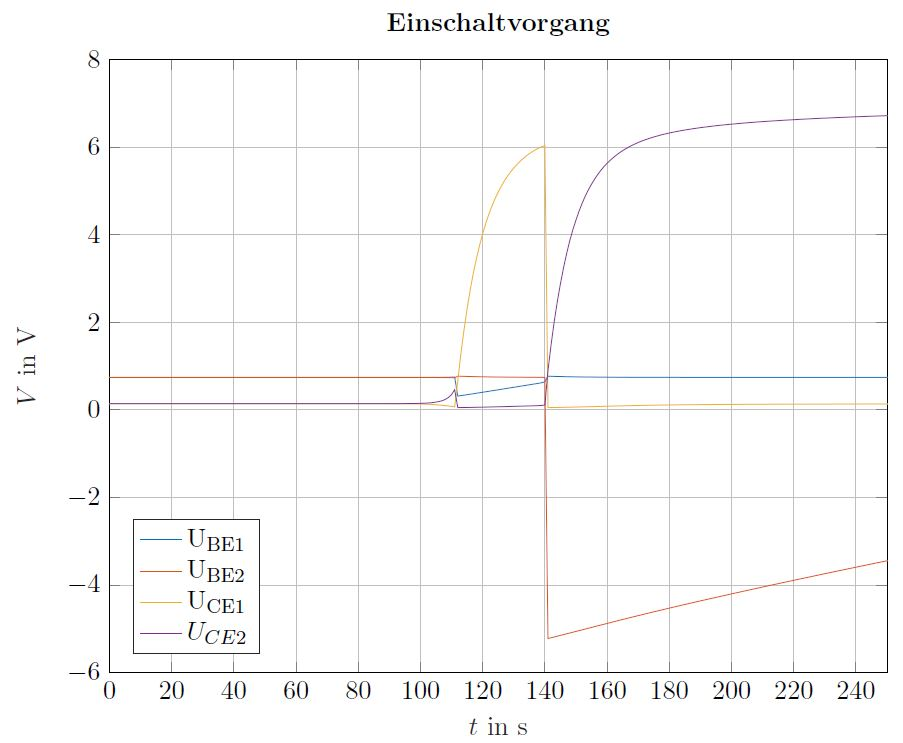
\includegraphics[width = 0.8\textwidth]{\figpath/Einschalt.jpg}
	\caption{Spannungen während Einschaltvorgang}
	\label{fig_Kap3_04:Einschalt}
\end{figure}

\begin{figure}[H]
	\centering \small
	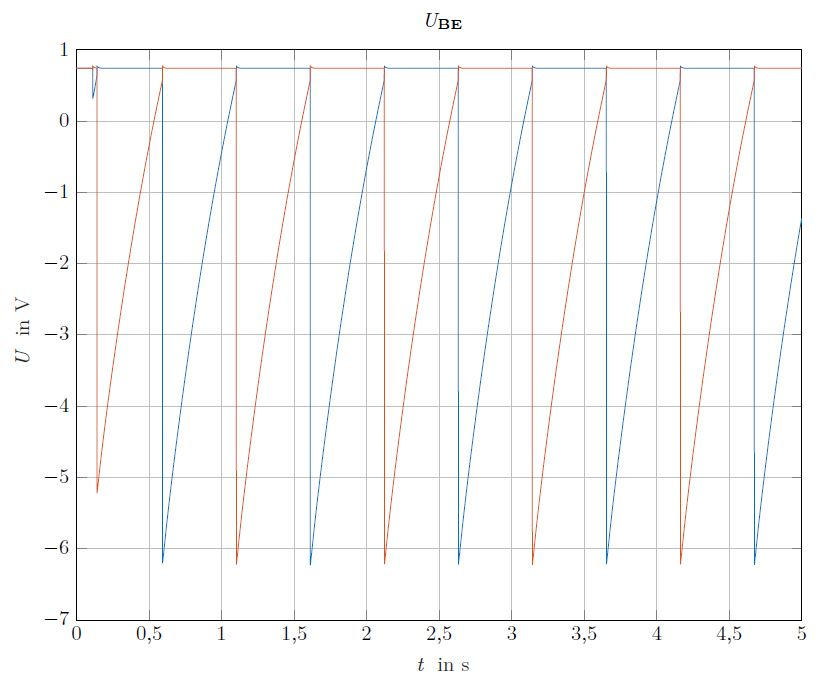
\includegraphics[width = 0.8\textwidth]{\figpath/U_BE.jpg}
	\caption{Basis-Emitter-Spannungen}
	\label{fig_Kap3_05:U_BE}
\end{figure}

\begin{figure}[H]
	\centering \small
	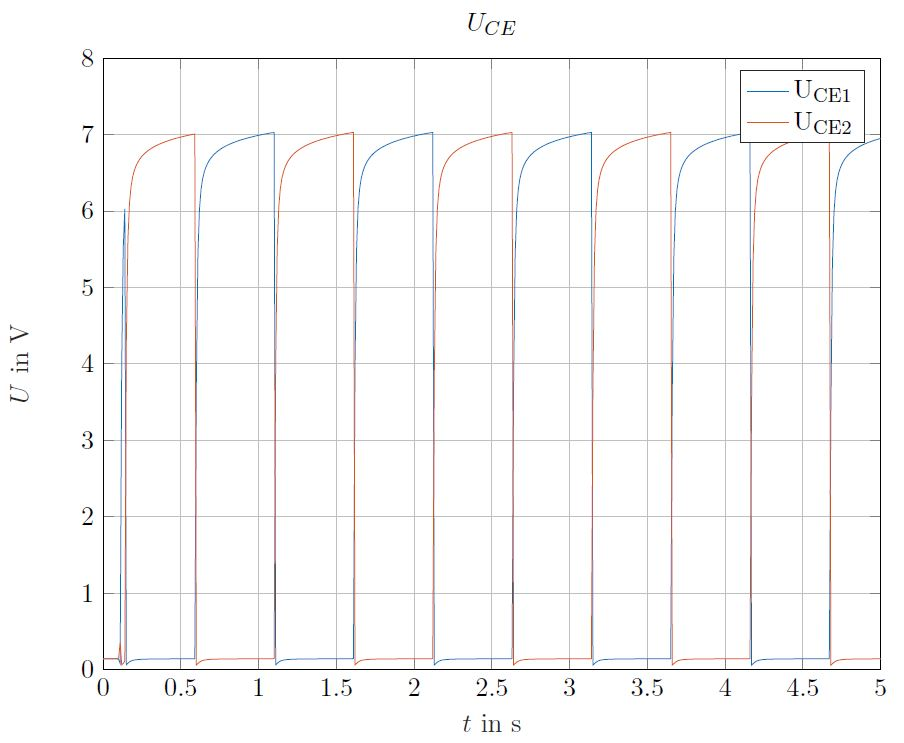
\includegraphics[width = 0.8\textwidth]{\figpath/U_CE.jpg}
	\caption{Kollektor-Emitter-Spannungen}
	\label{fig_Kap3_06:U_CE}
\end{figure}

\begin{figure}[H]
	\centering \small
	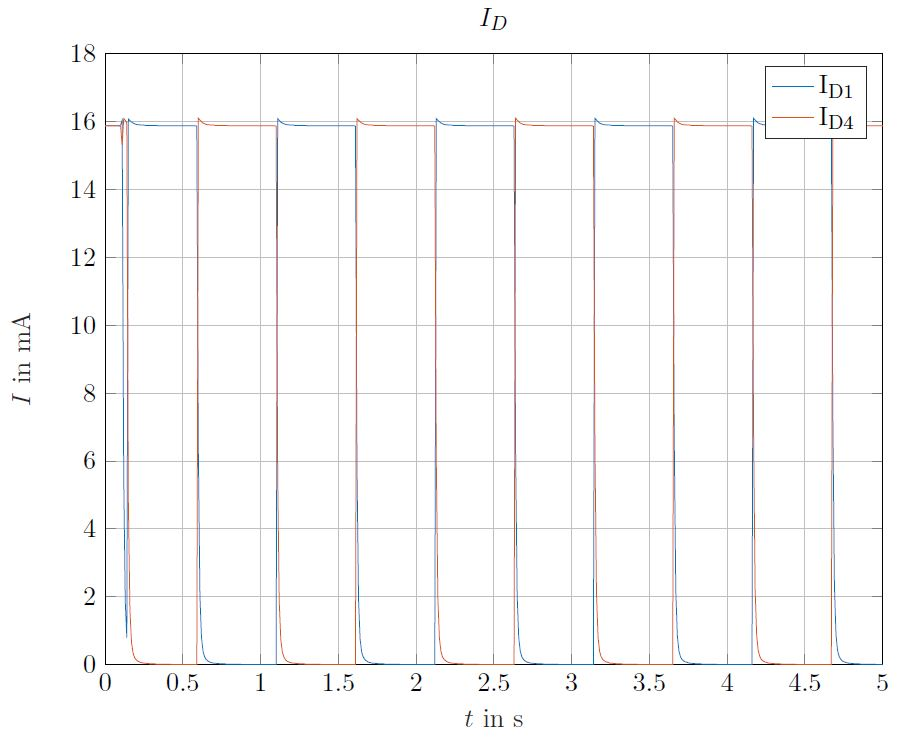
\includegraphics[width = 0.8\textwidth]{\figpath/I_D.jpg}
	\caption{Diodenströme}
	\label{fig_Kap3_07:I_D}
\end{figure}

Die Abbildungen zeigen, dass die Überschlagsrechnung für die Periodendauer bzw. die einzelnen Schaltzyklen, siehe Gleichung \ref{glgn:period}, gut mit der Simulation übereinstimmt.

Die Basis-Emitter-Spannung der Transistoren nimmt Werte bis ungefähr -6V an und hängt von der Versorgungsspannung ab. Damit die Basis-Emitter-Spannungen der Transistoren keine zu hohen negativen Werte annehmen, und die Transistoren damit vor Schädigung geschützt werden, können Dioden in Serie zur Transistor-Basis angebracht werden, siehe Abb. \ref{fig_Kap3_08:LTSpice_Schem_2}.

\begin{figure}[H]
    \centering
    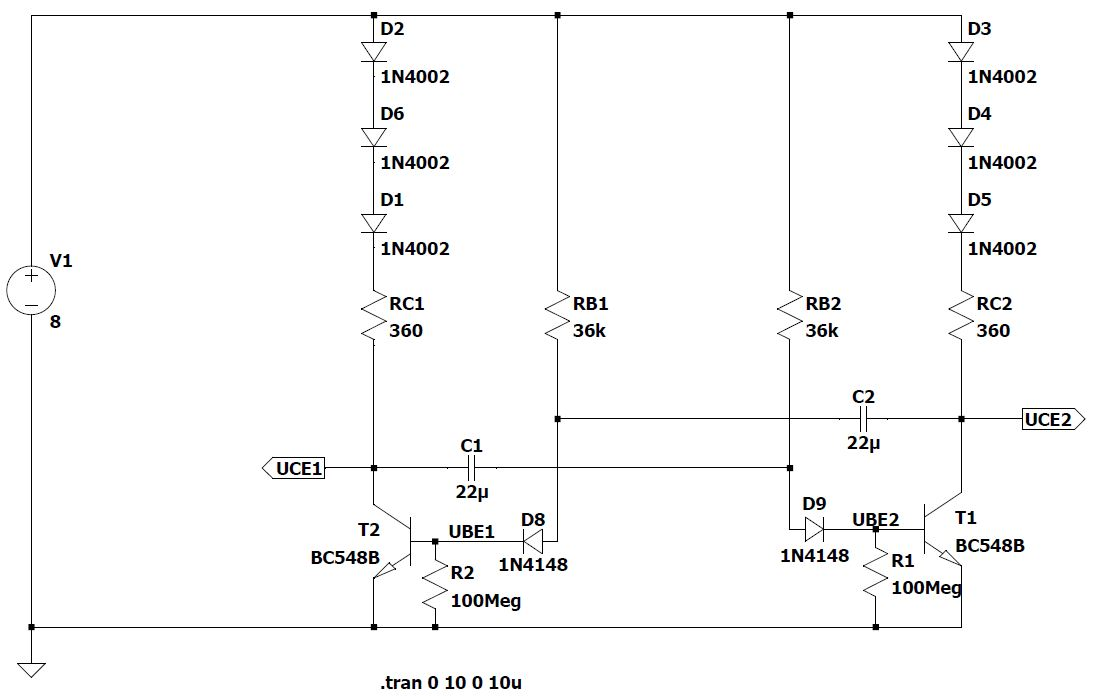
\includegraphics[width = 0.8\textwidth]{\figpath/Kipp_Schem_Diode.jpg}
    \caption{Astabile Kippschaltung in LTSpice mit Schutzdioden}
    \label{fig_Kap3_08:LTSpice_Schem_2}
\end{figure}

Die Basis-Emitter-Stufe ist sehr hochohmig, weswegen in der Simulation der Potentialbezug zur Masse verloren geht, wenn die Diode sperrt. Daher wurde auf beiden Seiten ein $\SI{100}{\mega\ohm}$ Widerstand eingefügt. Die Schaltung wurde 5 Sekunden lang mit Zeitschritten von $\SI{10}{\micro\second}$ simuliert. Die Spannungskurven können Abbildung \ref{fig_Kap3_09:Spannungen} entnommen werden.

\begin{figure}[H]
	\centering \small
	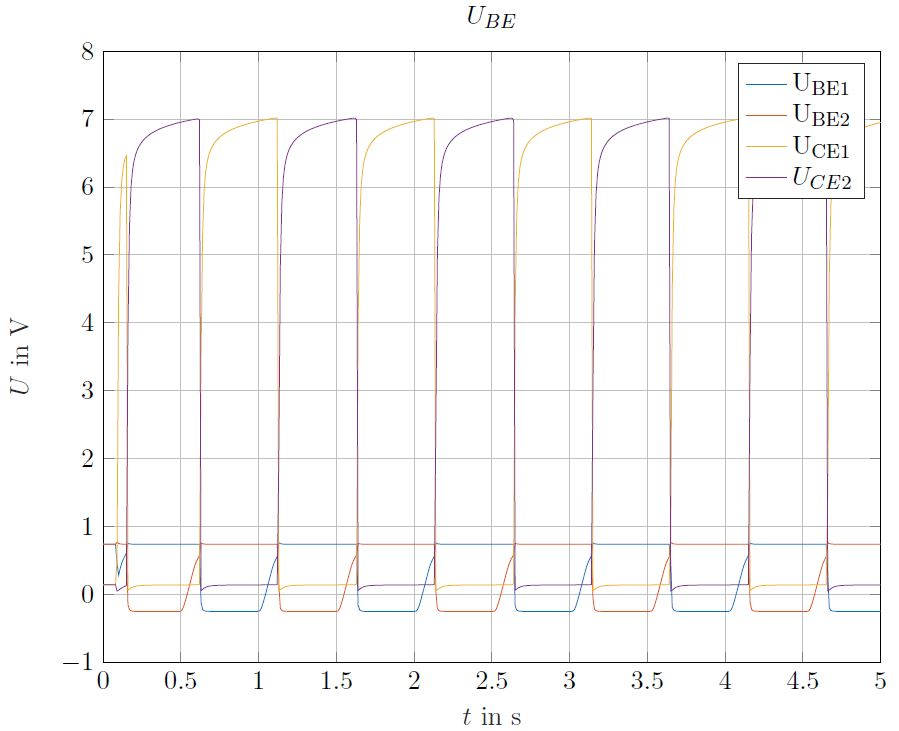
\includegraphics[width = 0.8\textwidth]{\figpath/U_diode.jpg}
	\caption{Spannungen der Astabilen Kippstufe mit Schutzdiode}
	\label{fig_Kap3_09:Spannungen}
\end{figure}

Durch die Sperrwirkung der Diode wird der Transistor im sicheren Bereich betrieben.

\section{Dreistufige Kippschaltung}
Als nächstes wird der astabile Monovibrator auf eine dreistufige Kippschaltung erweitert, siehe Abb. \ref{fig_Kap3_10:3stufig}. Die Schaltung wurde 5 Sekunden lang mit maximalen Zeitschritten von $\SI{10}{\micro\second}$ in LTSpice simuliert.

\begin{figure}[H]
    \centering
    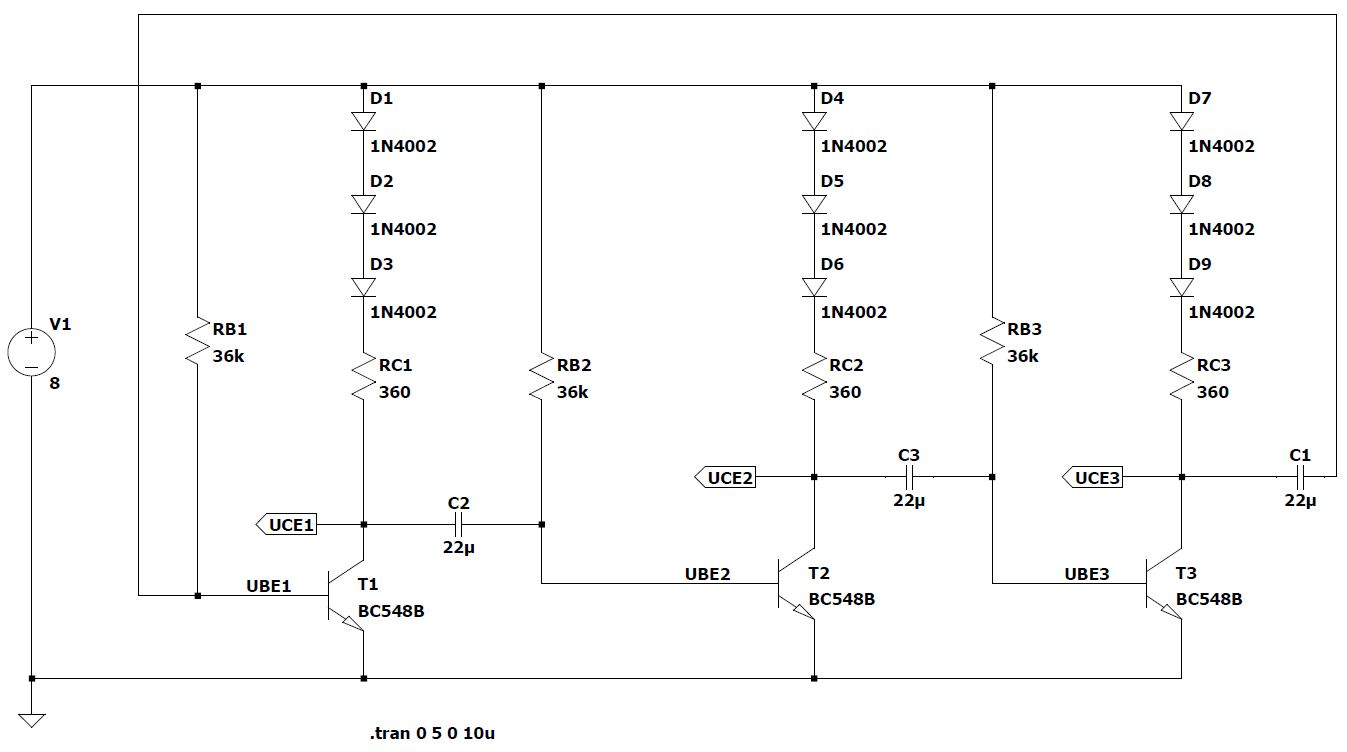
\includegraphics[width = 0.8\textwidth]{\figpath/Kipp_schem_3stufig.jpg}
    \caption{Blinkschaltung mit 3 LEDs}
    \label{fig_Kap3_10:3stufig}
\end{figure}

In Abb. \ref{fig_Kap3_11:Spannungen} können nun die Basis-Emitterspannungen der drei Transistoren betrachtet werden.

\begin{figure}[H]
	\centering \small
	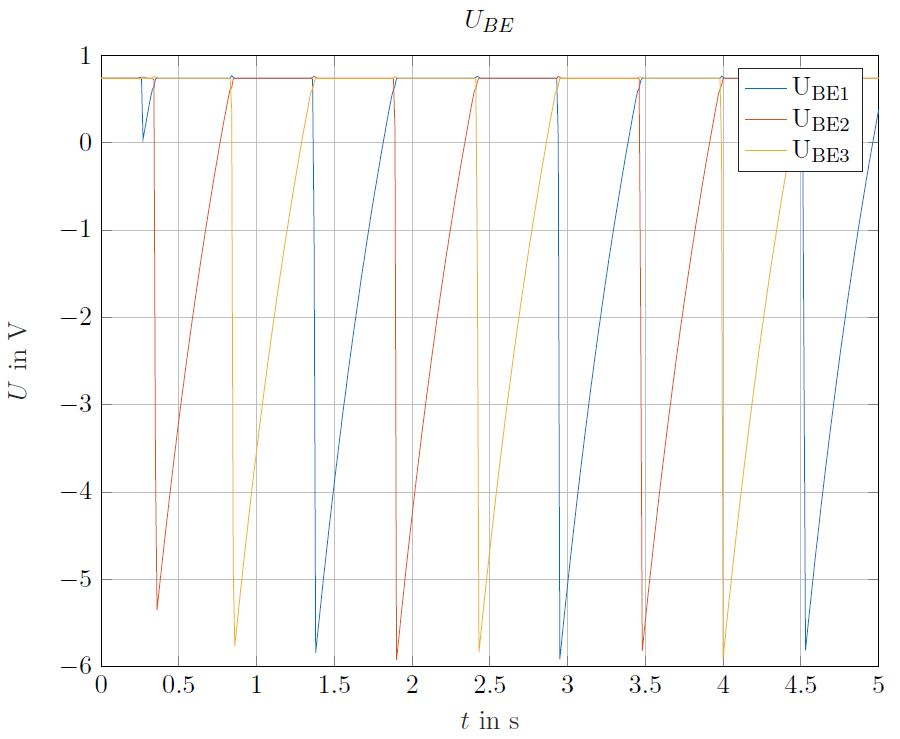
\includegraphics[width = 0.8\textwidth]{\figpath/U_3stufig.jpg}
	\caption{Basis-Emitter-Spannungen des 3-Stufigen LED-Blinklichts}
	\label{fig_Kap3_11:Spannungen}
\end{figure}

Anhand der Basis-Emitterspannungen erkennt man, das immer 2 Transistoren leiten, während einer sperrt. Die Dauer der einzelnen Schaltzustände ergibt sich wiederum aus den Ladevorgängen der Basisseitig angebrachten Kondensatoren und beträgt ca. $\SI{0,5}{\second}$. 

Will man erreichen, dass immer nur eine LED leuchtet, schaltet man einfach die LEDs mit einem geeignetem Vorwiderstand parallel zur Kollektor-Emitterstufe der npn-Transistoren, siehe Abb. \ref{fig_Kap3_111:Spannungen}.

\begin{figure}[H]
	\centering \small
	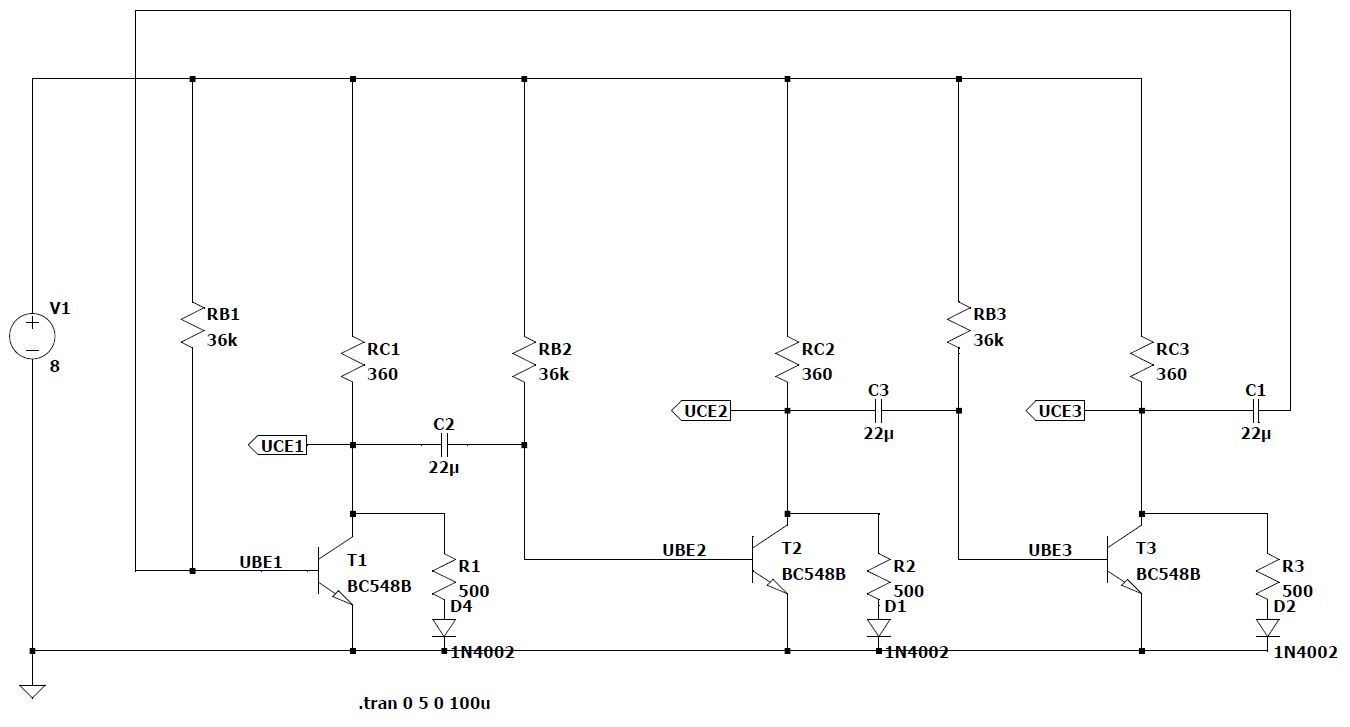
\includegraphics[width = 0.8\textwidth]{\figpath/Kipp_schem_3stufig_variation.jpg}
	\caption{Basis-Emitter-Spannungen des 3-Stufigen LED-Blinklichts}
	\label{fig_Kap3_111:Spannungen}
\end{figure}

Nun wird die Schaltung um eine Stufe erweitert, Abb. \ref{fig_Kap3_12:4stufig}.

\begin{figure}[H]
    \centering
    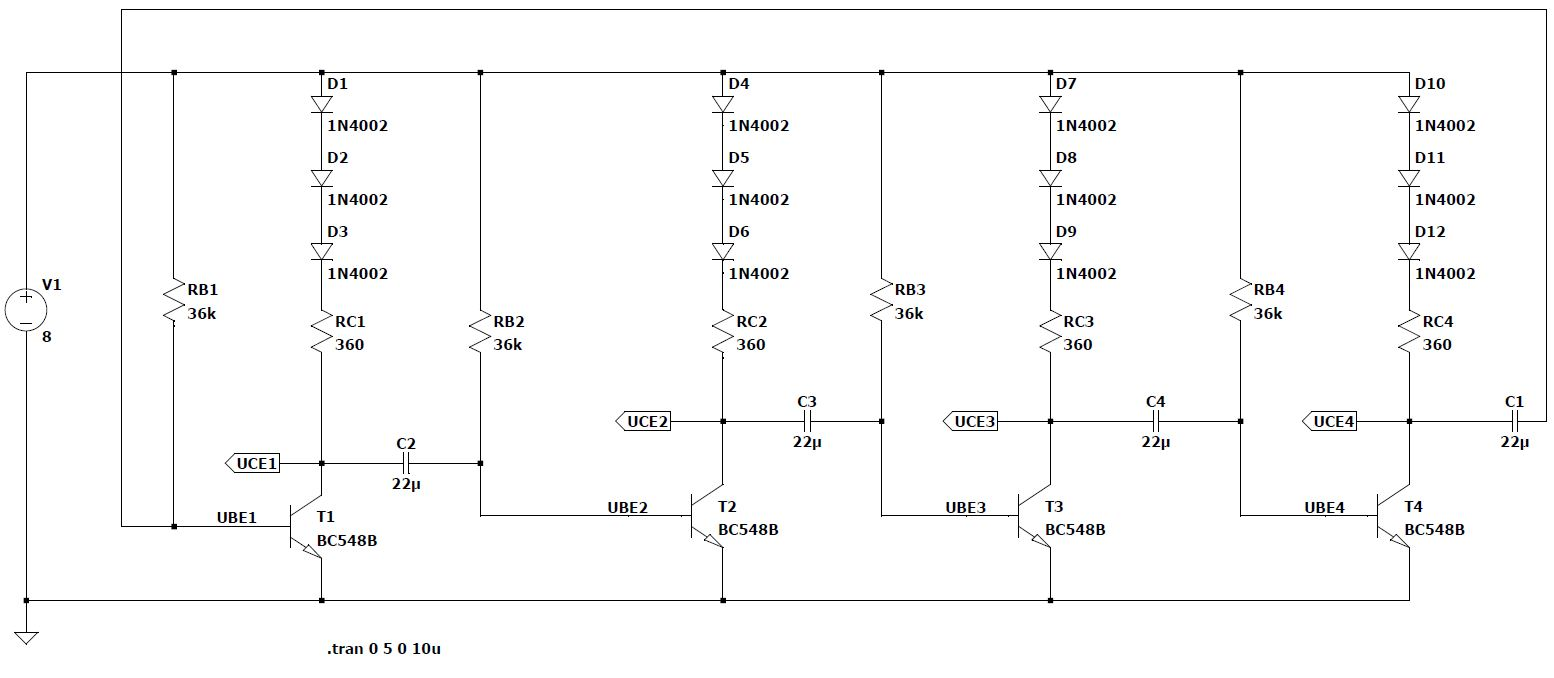
\includegraphics[width = \textwidth]{\figpath/Kipp_schem_4stufig.jpg}
    \caption{4 stufige Schaltung}
    \label{fig_Kap3_12:4stufig}
\end{figure}

\begin{figure}[H]
	\centering \small
	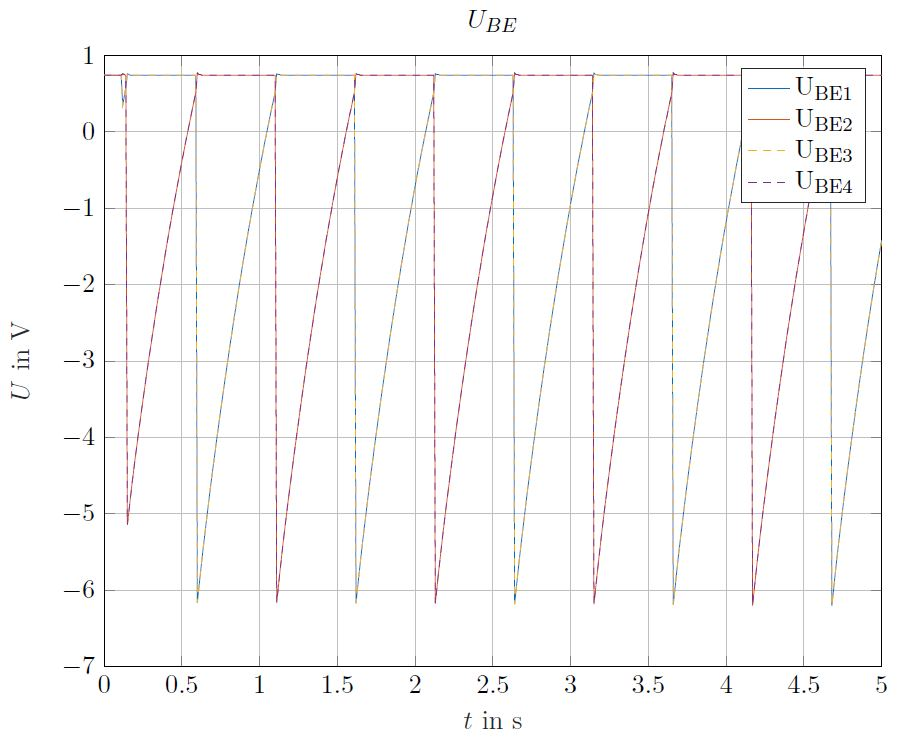
\includegraphics[width = 0.8\textwidth]{\figpath/U_4stufig.jpg}
	\caption{Basis-Emitter-Spannungen des 4-Stufigen LED-Blinklichts}
	\label{fig_Kap3_13:Spannungen}
\end{figure}

Die Schaltung funktioniert also nicht als 4-stufiges Lauflicht. Nun stellt sich die Frage, ob trotzdem eine Erweiterung auf 5 Stufen möglich ist, siehe Abb. \ref{fig_Kap3_14:5stufig}.

\begin{figure}[H]
    \centering
    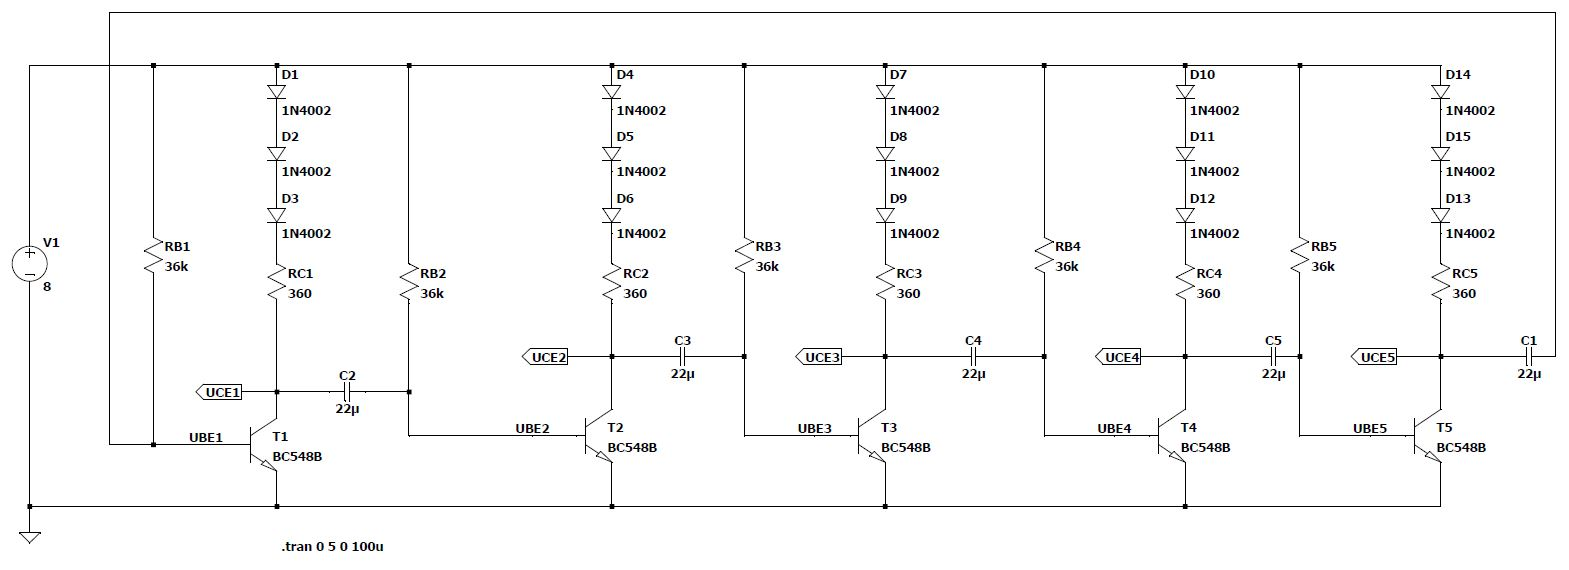
\includegraphics[width = \textwidth]{\figpath/Kipp_schem_5stufig.jpg}
    \caption{5 stufige Schaltung}
    \label{fig_Kap3_14:5stufig}
\end{figure}

\begin{figure}[H]
	\centering \small
	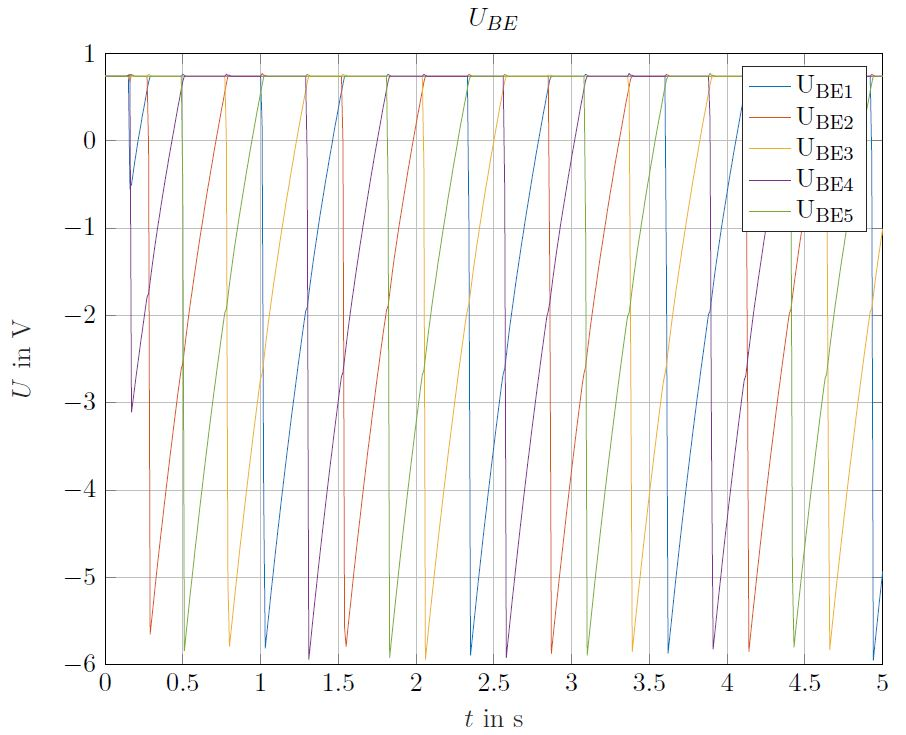
\includegraphics[width = 0.8\textwidth]{\figpath/U_5stufig.jpg}
	\caption{Basis-Emitter-Spannungen des 5-Stufigen LED-Blinklichts}
	\label{fig_Kap3_15:Spannungen}
\end{figure}

Lt. Spice-Simulation wäre eine Erweiterung auf 5 Stufen möglich, jedoch wird die Schaltung in Realität nicht so funktionieren.